\documentclass[12pt]{ximera}
\title{Exam 1}
\begin{document}
\begin{abstract}
Exam 1, covering Sections 7.1--7.3: De Morgan's laws and Venn diagram shading, set
operations, inclusion-exclusion, a three-set Venn diagram of pea-plant traits, and
equally likely outcomes from a pair of dice.
\end{abstract}
\maketitle

\section*{Exam 1}

Give your answers as exact fractions, decimals, or percentages; do not round unless
specifically asked to do so.

Formulas that may be useful:
\[
n(A\cup B) = n(A) + n(B) - n(A\cap B), \qquad
P(E) = \frac{n(E)}{n(S)}, \qquad
P\!\left(\olsi{E}\right)=1-P(E).
\]

\begin{problem}
Assess whether each of the following claims is true or false.

\begin{prompt}
\textbf{(a)} Claim: the union of the complements of two sets can be equivalently
written as the complement of their intersection. That is, for any sets $A$ and $B$,
\[ \olsi{A}\cup \olsi{B} = \olsi{A\cap B}. \]

\begin{multipleChoice}
\choice[correct]{True}
\choice{False}
\end{multipleChoice}

\begin{feedback}
True --- this is exactly one of De Morgan's laws.

In words: to be outside the overlap of $A$ and $B$, you must be missing from at least
one of them, which is to say you are in $\olsi{A}$ or in $\olsi{B}$.
\end{feedback}
\end{prompt}

\begin{prompt}
\textbf{(b)} Claim: the Venn diagram below shows the set
$\left(A\cup B\right)\cap \olsi{C}$.

\begin{center}
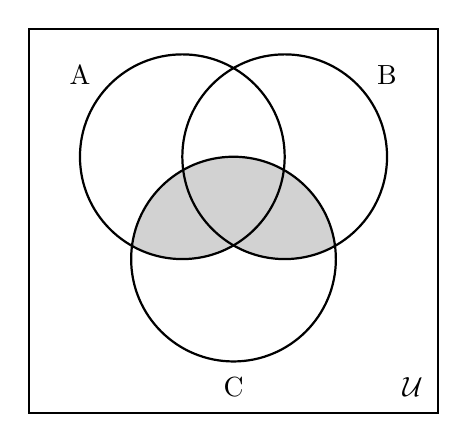
\begin{tikzpicture}[scale=1.3]
  \begin{scope}
    \clip (0.5,-1) circle (1);
    \fill[gray!35] (0,0) circle (1);
    \fill[gray!35] (1,0) circle (1);
  \end{scope}
  \draw[thick] (0,0) circle (1) node at (-1,0.8) {A};
  \draw[thick] (1,0) circle (1) node at (2,0.8) {B};
  \draw[thick] (0.5,-1) circle (1) node at (0.5,-2.25) {C};
  \draw[thick] (-1.5,-2.5) rectangle (2.5,1.25);
  \node at (2.25,-2.25) {$\mathcal{U}$};
\end{tikzpicture}
\end{center}

\begin{multipleChoice}
\choice{True}
\choice[correct]{False}
\end{multipleChoice}

\begin{hint}
Is the shaded region inside $C$ or outside $C$?
\end{hint}

\begin{feedback}
False. Every shaded point lies \emph{inside} $C$, so the diagram shows
\[ \left(A\cup B\right)\cap C, \]
not $\left(A\cup B\right)\cap\olsi{C}$. The claimed set would instead be the parts of
$A$ and $B$ that stick out of $C$ --- exactly the unshaded portions of those two
circles.
\end{feedback}
\end{prompt}
\end{problem}

\begin{problem}
Suppose $\mathcal{U}=\set{0,1,2,3,4,5,6,7,8,9,10}$. Consider the sets
\[
A= \set{0,2,4,6,8},\quad B= \set{0,3,6,9},\quad C= \set{1,2,3,4,5}.
\]

\begin{prompt}
\textbf{(a)} What is $n(A \cap B)$?

$\answer{2}$

\begin{feedback}
$A\cap B=\set{0,6}$, which has $2$ elements, so $n(A\cap B)=2$.
\end{feedback}
\end{prompt}

\begin{prompt}
\textbf{(b)} Write the set $\olsi{A\cup C}$ in proper set notation, listing its
elements explicitly. Enter them in increasing order.

$\olsi{A\cup C}=\set{\answer{7},\ \answer{9},\ \answer{10}}$

\begin{hint}
Build $A\cup C$ first, then take everything in $\mathcal{U}$ that is left over.
\end{hint}

\begin{feedback}
First,
\[ A\cup C=\set{0,2,4,6,8}\cup\set{1,2,3,4,5}=\set{0,1,2,3,4,5,6,8}. \]
The elements of $\mathcal{U}$ not in that union are $7$, $9$, and $10$, so
\[ \olsi{A\cup C}=\set{7,9,10}. \]
\end{feedback}
\end{prompt}
\end{problem}

\begin{problem}
Suppose that in a survey of $70$ students, $50$ report they like wallabies, $35$
report they like axolotls, and $65$ of the students report liking \emph{one or both}
of the creatures.

\begin{prompt}
\textbf{(a)} Use the Principle of Inclusion-Exclusion to determine how many students
report liking \emph{both} of these animals.

$\answer{20}$ students.

\begin{feedback}
Inclusion-exclusion gives $n(W\cup A)=n(W)+n(A)-n(W\cap A)$, so
\[ 65 = 50+35-n(W\cap A) = 85 - n(W\cap A), \]
and therefore $n(W\cap A)=85-65=20$.
\end{feedback}
\end{prompt}

\begin{prompt}
\textbf{(b)} What is the probability that a random student likes \emph{only}
wallabies?

Give your answer as a fraction in lowest terms: $\answer{3/7}$

\begin{hint}
``Only wallabies'' means the wallaby-likers with the both-likers removed.
\end{hint}

\begin{feedback}
Of the $50$ who like wallabies, $20$ also like axolotls, so $50-20=30$ like only
wallabies. Out of $70$ students,
\[ P(\text{only wallabies})=\frac{30}{70}=\frac{3}{7}\approx 0.429. \]
\end{feedback}
\end{prompt}
\end{problem}

\begin{problem}
After a genetics experiment involving $50$ pea plants, the plants that were tall
(T), had green peas (G), or had smooth peas (S) were each tallied, with the
following results:
\begin{itemize}
    \item $22$ were tall;
    \item $25$ had green peas;
    \item $9$ were tall with green peas;
    \item $20$ had smooth, green peas;
    \item $7$ were tall with smooth peas;
    \item $6$ were tall with smooth, green peas;
    \item $4$ were \emph{not} tall, with peas that were \emph{neither} green nor smooth.
\end{itemize}

\begin{prompt}
\textbf{(a)} Complete the Venn diagram.

\begin{center}
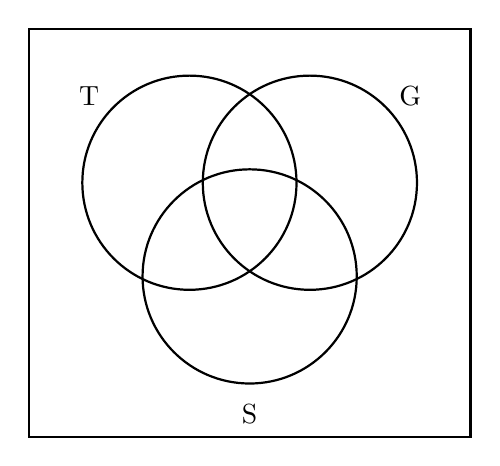
\begin{tikzpicture}[scale=0.85]
  \draw[thick] (-0.9,0.5) circle (1.6) node at (-2.4,1.8) {T};
  \draw[thick] (0.9,0.5) circle (1.6) node at (2.4,1.8) {G};
  \draw[thick] (0,-0.9) circle (1.6) node at (0,-2.95) {S};
  \draw[thick] (-3.3,-3.3) rectangle (3.3,2.8);
\end{tikzpicture}
\end{center}

All three: $\answer{6}$

\smallskip
T and G only: $\answer{3}$ \qquad
T and S only: $\answer{1}$ \qquad
G and S only: $\answer{14}$

\smallskip
T only: $\answer{12}$ \qquad
G only: $\answer{2}$ \qquad
S only: $\answer{8}$ \qquad
None: $\answer{4}$

\begin{hint}
Six regions follow directly from the given overlaps. The ``S only'' region is the one
you cannot get that way --- find it last, using the fact that all eight regions must
total $50$ plants.
\end{hint}

\begin{feedback}
Working outward from the center:
\begin{itemize}
\item All three: $6$, given.
\item T and G only: $9-6=3$. \quad T and S only: $7-6=1$. \quad
      G and S only: $20-6=14$.
\item T only: $22-(3+1+6)=12$. \quad G only: $25-(3+14+6)=2$.
\item None: $4$, given.
\end{itemize}
Those seven regions total $6+3+1+14+12+2+4=42$. Since there are $50$ plants
altogether, the remaining region --- smooth only --- contains $50-42=8$ plants.

Note that the total number of smooth-pea plants was never given directly; it has to
be recovered from the grand total of $50$.
\end{feedback}
\end{prompt}

\begin{prompt}
\textbf{(b)} How many of the pea plants were \emph{not} tall and had peas that were
\emph{not} green but \emph{were} smooth?

$\answer{8}$ plants.

\begin{feedback}
This describes the ``smooth only'' region, which part (a) found to be
$50-42=8$ plants.
\end{feedback}
\end{prompt}

\begin{prompt}
\textbf{(c)} How many of the pea plants had smooth peas, altogether?

$\answer{29}$ plants.

\begin{feedback}
Add the four regions inside the S circle:
\[ 8 + 1 + 14 + 6 = 29 \text{ plants.} \]
\end{feedback}
\end{prompt}

\begin{prompt}
\textbf{(d)} Based on the data given above, what are the \emph{odds} that a random pea
plant from this experiment has smooth, green peas? Reduce your answer.

The odds are $\answer{2}$ to $\answer{3}$.

\begin{feedback}
The plants with both smooth and green peas are the ``G and S only'' region plus the
center: $14+6=20$. The other $50-20=30$ plants do not have both traits. So the odds
are
\[ 20:30 = 2:3. \]
\end{feedback}
\end{prompt}
\end{problem}

\begin{problem}
You're playing a version of D\&D where whenever your character attacks, you roll a
d12 (12-sided die) and a d6 (6-sided die). The d12 result determines whether the
attack hits, and the d6 result determines how much damage is dealt.

Suppose for a particular opponent, you need to roll at least an $8$ on the d12 to
hit, and if you both hit and deal more than $4$ damage then you will have defeated
them.

\begin{prompt}
\textbf{(a)} If we record the result of both rolls, how many equal-probability
outcomes are there altogether?

$\answer{72}$

\begin{hint}
Imagine a table with one row per d12 result and one column per d6 result.
\end{hint}

\begin{feedback}
By the multiplication principle, there are
\[ 12\cdot 6 = 72 \]
equally likely $(\text{d12},\text{d6})$ pairs.
\end{feedback}
\end{prompt}

\begin{prompt}
\textbf{(b)} What is the probability that your attack hits?

Give your answer as a fraction in lowest terms: $\answer{5/12}$

\begin{feedback}
A hit means the d12 shows $8$, $9$, $10$, $11$, or $12$ --- five of its twelve faces.
So
\[ P(\text{hit})=\frac{5}{12}. \]
(Counting outcome pairs instead gives $\frac{5\cdot 6}{72}=\frac{30}{72}=\frac{5}{12}$,
the same answer.)
\end{feedback}
\end{prompt}

\begin{prompt}
\textbf{(c)} What is the probability that your attack hits \emph{and} deals more than
$4$ damage?

Give your answer as a fraction in lowest terms: $\answer{5/36}$

\begin{hint}
``More than $4$'' on a d6 means a $5$ or a $6$. The two dice are independent.
\end{hint}

\begin{feedback}
More than $4$ damage means the d6 shows $5$ or $6$, which has probability
$\frac26=\frac13$. The dice are independent, so
\[
P(\text{hit and}>4)=\frac{5}{12}\cdot\frac13=\frac{5}{36}.
\]
Equivalently, $5\cdot 2=10$ of the $72$ outcome pairs qualify, and
$\frac{10}{72}=\frac{5}{36}$.
\end{feedback}
\end{prompt}

\begin{prompt}
\textbf{(d)} A result of $12$ on the d12 is called a ``critical hit'' and will defeat
the opponent regardless of the damage roll. What is the probability that \emph{either}
you roll a $12$ on the d12 \emph{or} you roll a hit with more than $4$ damage?

Give your answer as a fraction in lowest terms: $\answer{7/36}$

\begin{hint}
These two events overlap --- rolling a $12$ together with a $5$ or $6$ satisfies both.
Use inclusion-exclusion so you do not count that overlap twice.
\end{hint}

\begin{feedback}
Count outcome pairs out of $72$.
\begin{itemize}
\item Critical hit: d12 $=12$ with any d6, which is $6$ pairs.
\item Hit with more than $4$ damage: $5$ d12 values by $2$ d6 values, which is $10$ pairs.
\item Both at once: d12 $=12$ and d6 $\in\set{5,6}$, which is $2$ pairs.
\end{itemize}
By inclusion-exclusion, the number of favorable pairs is $6+10-2=14$, so
\[
P = \frac{14}{72} = \frac{7}{36}\approx 0.194.
\]
The subtraction matters here: adding $\frac{1}{12}+\frac{5}{36}=\frac{8}{36}$ would
double-count the two outcomes that are both a critical hit and a high-damage hit.
\end{feedback}
\end{prompt}
\end{problem}

\end{document}
